\documentclass[12pt, a4paper] {ncc}
\usepackage[utf8] {inputenc}
\usepackage[T2A]{fontenc}
\usepackage[english, russian] {babel}
\usepackage[usenames,dvipsnames]{xcolor}
\usepackage{listings,a4wide,longtable,amsmath,amsfonts,graphicx,tikz}
\usepackage{indentfirst}
\usepackage{bytefield}
\usepackage{multirow}
\usepackage{float}
\usepackage{caption}
\usepackage{subcaption}
\captionsetup{compatibility=false}
\usepackage{tabularx}

\usepackage[left=2cm,right=2cm,top=2cm,bottom=2cm,bindingoffset=0cm]{geometry}

\begin{document}
\setcounter{figure}{0}
\frenchspacing
\pagestyle{empty}
\begin{center}
							Университет ИТМО	\\
                        Кафедра вычислительной техники

\vspace{\stretch{2}}
                    Методы цифровой обработки сигналов
\end{center}
\vspace{\stretch{2}}
\begin{center}
                            Лабораторная работа №2\\
						{\bf Исследование эффективности метода подавления низкочастных помех
							 с помощью усредняющего фильтра}
\end{center}
\vspace{\stretch{3}}
\begin{flushright}
                                    Студент:\\
                                    {\it Куклина Мария, P3401}\\
									Преподаватель: \\
									{\it Тропченко А.А.}
\end{flushright}
\vspace{\stretch{4}}
\begin{center}
                             Санкт-Петербург, 2017
\end{center}
\newpage


\section{Цели работы}
    Определение возможностей метода подавления низкочастных помех с помощью
	линейного фильтра.

\section{Задание}

    \begin{description}
        \item[Частота сигнала:] $8$.
        \item[Амплитуда сигнала:] $1$.
        \item[Частота помехи:]  $0.2-2$.
        \item[Амплитуда помехи:] $40$.
    \end{description}


\section{Исследование зависимости соотношения SNR в выходной смеси от соотношения частот SNR}
    
        \begin{table}[H]
            \centering
            \begin{tabular} { |c|c|c| }
                \hline
                \textbf{$F_r$} & \textbf{$ \frac {F_r} {F_s} $} & \textbf{SNR}  \\ \hline
                    0.2 & 75     &   123.9288 \\ \hline
                    0.3 & 50     &   66.6692  \\ \hline
                    0.4 & 37.5   &   38.4643  \\ \hline
                    0.5 & 30     &   22.2021  \\ \hline
                    0.6 & 25     &   14.4936  \\ \hline
                    0.7 & 21.42  &   10.9197  \\ \hline
                    0.8 & 18.75  &   8.9080   \\ \hline
                    0.9 & 16.66  &   7.1767   \\ \hline
                    1   & 15     &   5.594    \\ \hline
                    1.1 & 13.63  &   4.489    \\ \hline
                    1.2 & 12.5   &   3.84     \\ \hline
                    1.3 & 11.53  &   3.428    \\ \hline
                    1.4 & 10.714 &   3.031    \\ \hline
                    1.5 & 10     &   2.61     \\ \hline
                    1.6 & 9.375  &   2.286    \\ \hline
                    1.7 & 8.8235 &   2.069    \\ \hline
                    1.8 & 8.333  &   1.9187   \\ \hline
                    1.9 & 7.89   &   1.7699   \\ \hline
                    2   & 7.5    &   1.611    \\ \hline
            \end{tabular}
        \end{table}

        \begin{figure}[H]
            \centering
            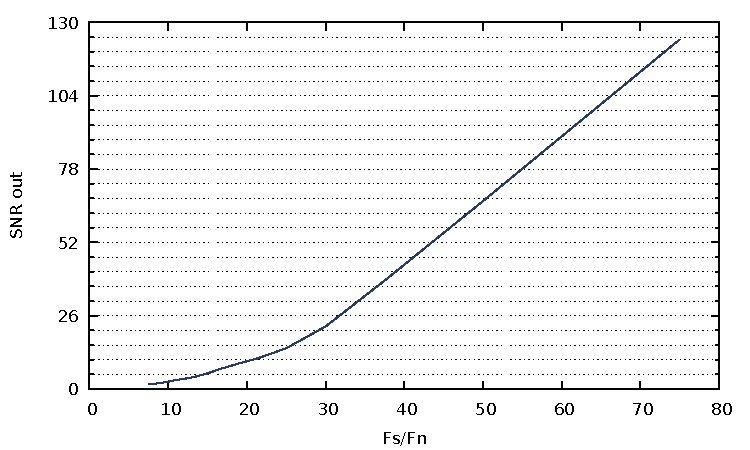
\includegraphics[scale=0.9,page=1]{snr_freq.pdf}
            \caption{Зависимость SNT от соотношения $\frac {F_r} {F_S}$ частот SNR}
        \end{figure}

\section{Исследование соотношения SNR на выхода от соотношения $\frac {A_r} {A_s}$ амплитуд помехи и сигнала}
        \begin{table}[H]
            \centering
            \begin{tabular} { |c|c|c| }
                \hline
                \textbf{$F_r$} & \textbf{$\frac{A_r} {A_s}$} & \textbf{SNR} \\ \hline
                     0.2	   & 40  & 123.928 \\ \hline
                     0.2	   & 100 & 49.5730 \\ \hline
                     0.2	   & 150 & 33.0523 \\ \hline
                     0.2	   & 200 & 24.7938 \\ \hline
                     0.2	   & 250 & 19.8402 \\ \hline
                     0.2	   & 300 & 16.5391 \\ \hline
                     0.2	   & 350 & 14.1822 \\ \hline
                     0.2	   & 400 & 12.4155 \\ \hline
                     0.2	   & 450 & 11.0423 \\ \hline
                     0.2	   & 500 & 9.9444 \\ \hline 
            \end{tabular}
            \begin{tabular} { |c|c|c| }
                \hline
                \textbf{$F_r$} & \textbf{$\frac{A_r} {A_s}$} & \textbf{SNR} \\ \hline
						0.8 &  40  & 8.9 \\ \hline
						0.8 &  100 & 3.645 \\ \hline
						0.8 &  150 & 2.51 \\ \hline
						0.8 &  200 & 1.9635 \\ \hline
						0.8 &  250 & 1.6489 \\ \hline
						0.8 &  300 & 1.4485 \\ \hline
						0.8 &  350 & 1.31174 \\ \hline
						0.8 &  400 & 1.2136 \\ \hline
						0.8 &  450 & 1.1405 \\ \hline
						0.8 &  500 & 1.0843 \\ \hline
            \end{tabular}
            \begin{tabular} { |c|c|c| }
                \hline
                \textbf{$F_r$} & \textbf{$\frac{A_r} {A_s}$} & \textbf{SNR} \\ \hline
                        1.4 &  40  & 3.03 \\ \hline
                        1.4 &  100 & 1.4402 \\ \hline
                        1.4 &  150 & 1.138 \\ \hline
                        1.4 &  200 & 1.005 \\ \hline
                        1.4 &  250 & 0.9321 \\ \hline
                        1.4 &  300 & 0.887 \\ \hline
                        1.4 &  350 & 0.8567 \\ \hline
                        1.4 &  400 & 0.8349 \\ \hline
                        1.4 &  450 & 0.8186 \\ \hline
                        1.4 &  500 & 0.806 \\ \hline
            \end{tabular}
            \begin{tabular} { |c|c|c| }
                \hline
                \textbf{$F_r$} & \textbf{$\frac{A_r} {A_s}$} & \textbf{SNR} \\ \hline
                    2 & 40  & 1.611 \\ \hline
                    2 & 100 & 0.974 \\ \hline
                    2 & 150 & 0.8652 \\ \hline
                    2 & 200 & 0.8172 \\ \hline
                    2 & 250 & 0.7906 \\ \hline
                    2 & 300 & 0.7737 \\ \hline
                    2 & 350 & 0.7622 \\ \hline
                    2 & 400 & 0.7538 \\ \hline
                    2 & 450 & 0.7474 \\ \hline
                    2 & 500 & 0.7424 \\ \hline
            \end{tabular}
        \end{table}

        \begin{figure}[H]
            \centering
            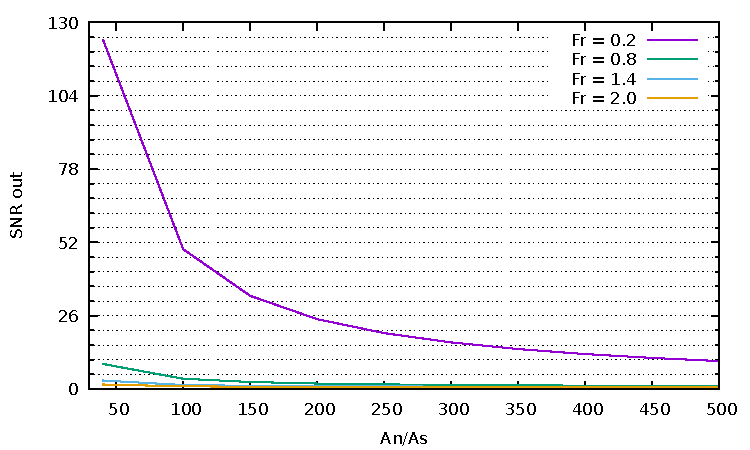
\includegraphics[scale=0.9,page=1]{snr_amp.pdf}
			\caption{соотношения SNR на выхода от соотношения $\frac {A_r} {A_s}$ амплитуд помехи и сигнала для фиксированных значений частоты помехи}
        \end{figure}

\section*{Функциональная схема устройства}
        \begin{figure}[H]
            \centering
            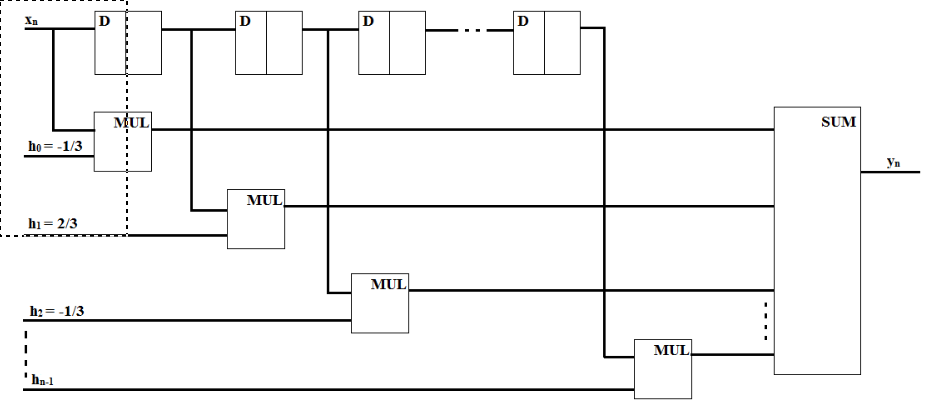
\includegraphics[scale=0.5,page=1]{schema.png}
        \end{figure}

\section*{Вывод}

В результате выполнения лабораторной работы были сделаны следующие выводы.


\end{document}
